\documentclass[11pt,a4paper]{article}
\usepackage{amsmath,amssymb,amsthm}
\usepackage{graphicx}
\usepackage[margin=2.2cm]{geometry}
\usepackage{xcolor}
\usepackage{titlesec}
\usepackage{fancyhdr}
\usepackage{booktabs}
\usepackage{enumitem}
\usepackage{float}
\usepackage{hyperref}
\hypersetup{colorlinks=true,linkcolor=blue!70!black,urlcolor=blue!70!black}

\renewcommand{\topfraction}{0.9}
\renewcommand{\bottomfraction}{0.9}
\renewcommand{\textfraction}{0.05}
\renewcommand{\floatpagefraction}{0.5}
\setcounter{topnumber}{3}
\setcounter{bottomnumber}{3}
\setcounter{totalnumber}{5}

\definecolor{primary}{RGB}{0,51,102}
\definecolor{accent}{RGB}{204,102,0}

\titleformat{\section}{\Large\bfseries\color{primary}}{\thesection}{1em}{}
\titleformat{\subsection}{\large\bfseries\color{primary!80!black}}{\thesubsection}{1em}{}

\pagestyle{fancy}
\fancyhf{}
\fancyhead[L]{\small\color{primary}Essential Summary}
\fancyhead[R]{\small\color{primary}Li et al.\ (2011)}
\fancyfoot[C]{\thepage}
\renewcommand{\headrulewidth}{0.5pt}

\begin{document}
\raggedbottom

\begin{center}
{\LARGE\bfseries\color{primary}Essential Summary}\\[12pt]
{\large\bfseries Generalized Projective Synchronization of\\Chaotic Systems via Modified Active Control}\\[8pt]
{\normalsize Zhenbo Li, Xiaoshan Zhao, Jing Wang}\\[4pt]
{\small\itshape Acta Physica Sinica, Vol.\ 60, No.\ 5, 050508 (2011)\\DOI: 10.7498/aps.60.050508}\\[6pt]
{\small\rule{0.7\textwidth}{0.5pt}}\\[4pt]
{\small\color{accent}This is an author-prepared essential summary, not the original paper.\\Please cite the published version.}
\end{center}

\vspace{0.5em}

\section{Background and Motivation}

Since Pecora and Carroll's 1990 demonstration of chaos synchronization, the field has grown into a rich hierarchy of synchronization types --- complete, phase, lag, generalized, and projective synchronization. \textbf{Generalized projective synchronization (GPS)} stands out because it relaxes two constraints of earlier projective synchronization: the systems no longer need to be partially linear, and the drive and response systems need not share the same structure. The defining feature of GPS is a projection matrix $\alpha I$: the response state converges to a \emph{scaled} replica of the drive state.

\begin{equation}
\lim_{t\to\infty}\lVert \mathbf{e}(t)\rVert = \lim_{t\to\infty}\lVert \mathbf{x}_m(t) - \alpha\mathbf{x}_s(t)\rVert = 0
\label{eq:gps}
\end{equation}

The scaling factor $\alpha$ allows arbitrary ``compression'' ($|\alpha|<1$) or ``stretching'' ($|\alpha|>1$) of the drive signal, in-phase ($\alpha>0$) or anti-phase ($\alpha<0$). This tunable property makes GPS attractive for digital secure communications.

The classical \textbf{active control} approach builds the controller matrix $M$ by requiring all eigenvalues of the closed-loop matrix $E-M$ to have negative real parts --- the \textbf{Routh--Hurwitz criterion}. For high-dimensional systems, computing these eigenvalues is expensive and error-prone. This paper proposes a \textbf{modified active control} method that replaces eigenvalue analysis with a \textbf{special matrix construction} validated directly by Lyapunov stability theory, thereby eliminating the Routh--Hurwitz dependence entirely.

\section{Problem Formulation}

Consider the drive system
\begin{equation}
\dot{\mathbf{x}}_m = A\mathbf{x}_m + Bf(\mathbf{x}_m),
\label{eq:drive}
\end{equation}
and the response system
\begin{equation}
\dot{\mathbf{x}}_s = C\mathbf{x}_s + Dg(\mathbf{x}_s) + \mathbf{u},
\label{eq:response}
\end{equation}
where $A,B,C,D$ are constant matrices, $f,g$ are nonlinear maps, and $\mathbf{u}$ is the controller to be designed. Define the error $\mathbf{e} = \mathbf{x}_m - \alpha\mathbf{x}_s$. Subtracting Eq.~\eqref{eq:response} from Eq.~\eqref{eq:drive} yields the error system
\begin{equation}
\dot{\mathbf{e}} = E\mathbf{e} + Kh(\mathbf{x}_m,\mathbf{x}_s,\alpha) - \alpha\mathbf{u},
\label{eq:error}
\end{equation}
with constant matrices $E,K$ and nonlinear residual $h$. GPS is achieved if a controller $\mathbf{u}$ renders the origin of Eq.~\eqref{eq:error} asymptotically stable.

\section{Modified Active Control}

\subsection{Controller Structure}

The controller is decomposed as $\mathbf{u} = \mathbf{u}_a + \mathbf{u}_b$:
\begin{equation}
\boxed{\mathbf{u}_a = \alpha^{-1} M\mathbf{e}, \qquad \mathbf{u}_b = \alpha^{-1} Kh(\mathbf{x}_m,\mathbf{x}_s,\alpha)}
\label{eq:controller}
\end{equation}
The component $\mathbf{u}_b$ cancels the nonlinear residual $K h$, while $\mathbf{u}_a$ shapes the linear part. Substituting Eq.~\eqref{eq:controller} into Eq.~\eqref{eq:error} collapses the error dynamics to the linear system
\begin{equation}
\dot{\mathbf{e}} = (E - M)\,\mathbf{e}.
\label{eq:closedloop}
\end{equation}

\subsection{Special Matrix Construction (Key Idea)}

The classical method requires $\lambda(E-M)\subset\mathbb{C}^-$ (Routh--Hurwitz). The modified method instead chooses $M$ so that the closed-loop matrix $N = E - M$ satisfies \textbf{only}:

\begin{itemize}[leftmargin=2em]
\item $n_{ij} = -n_{ji}$ for $i\neq j$ (skew-symmetric off-diagonal blocks),
\item $n_{ii} \leq 0$, not all zero (non-positive diagonal),
\item there exist positive weights $k_i > 0$.
\end{itemize}

\textbf{Why this works:} choose the Lyapunov function
\begin{equation}
V = \sum_{i=1}^{n}\frac{e_i^2}{k_i},
\qquad
\dot{V} = 2\sum_{i=1}^{n}\frac{n_{ii}}{k_i}e_i^2 \;\leq\; 0,
\label{eq:lyap}
\end{equation}
so asymptotic stability follows immediately without any eigenvalue computation. For high-dimensional systems this is dramatically simpler than Routh--Hurwitz.

\section{Example 1: Self-Structure Synchronization (Energy Resource System)}

The energy demand--supply system (describing the coupled relationship between Jiangsu's energy demand and Western energy supply) is used as both drive and response:

\begin{equation}
\dot{x}_m = a_1 x_m[1 - x_m/M] - a_2(y_m+z_m),
\qquad
\dot{y}_m = -b_1 y_m - b_2 z_m + b_3 x_m[N - (x_m-z_m)],
\qquad
\dot{z}_m = c_1 z_m(c_2 x_m - c_3),
\label{eq:energy}
\end{equation}
with $a_1=0.09,\ a_2=0.15,\ b_1=0.06,\ b_2=0.082,\ b_3=0.07,\ c_1=0.2,\ c_2=0.5,\ c_3=0.4,\ M=1.8,\ N=1$. The resulting chaotic attractor is shown in Figure~\ref{fig:fig1}.

\begin{figure}[htbp]
\centering
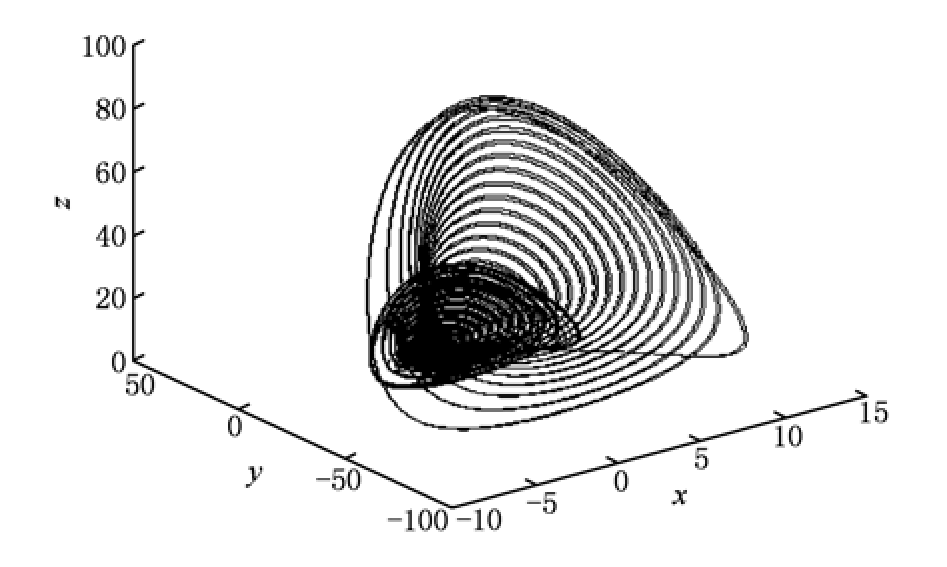
\includegraphics[width=0.8\textwidth,height=0.4\textheight,keepaspectratio]{aps2011-fig1.png}
\caption{Three-dimensional chaotic phase portrait of the energy resource system Eq.~\eqref{eq:energy}.}
\label{fig:fig1}
\end{figure}

For $\alpha=-2$ (anti-phase compression) and $\alpha=3$ (in-phase compression), the controller Eq.~\eqref{eq:controller} with $k_1=1,\ k_2=5,\ k_3=10$ drives the error to zero, as shown in Figures~\ref{fig:fig2}--\ref{fig:fig3}.

\begin{figure}[htbp]
\centering
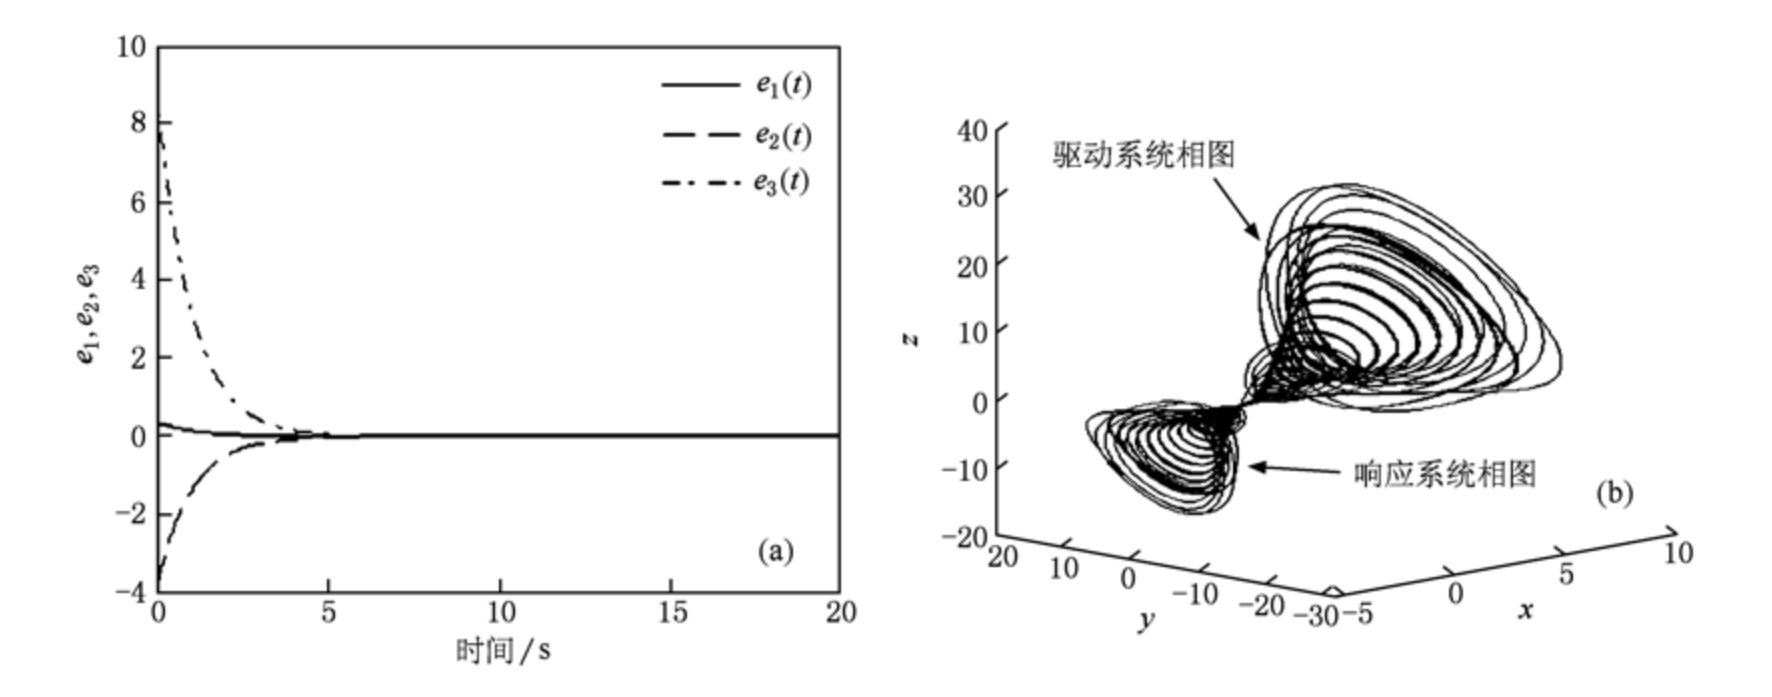
\includegraphics[width=0.9\textwidth,height=0.42\textheight,keepaspectratio]{aps2011-fig2.png}
\caption{(a) Synchronization error curves for $\alpha=-2$; (b) three-dimensional GPS phase portraits of drive and response systems for $\alpha=-2$. The response phase portrait is an anti-phase compressed replica of the drive.}
\label{fig:fig2}
\end{figure}

\begin{figure}[htbp]
\centering
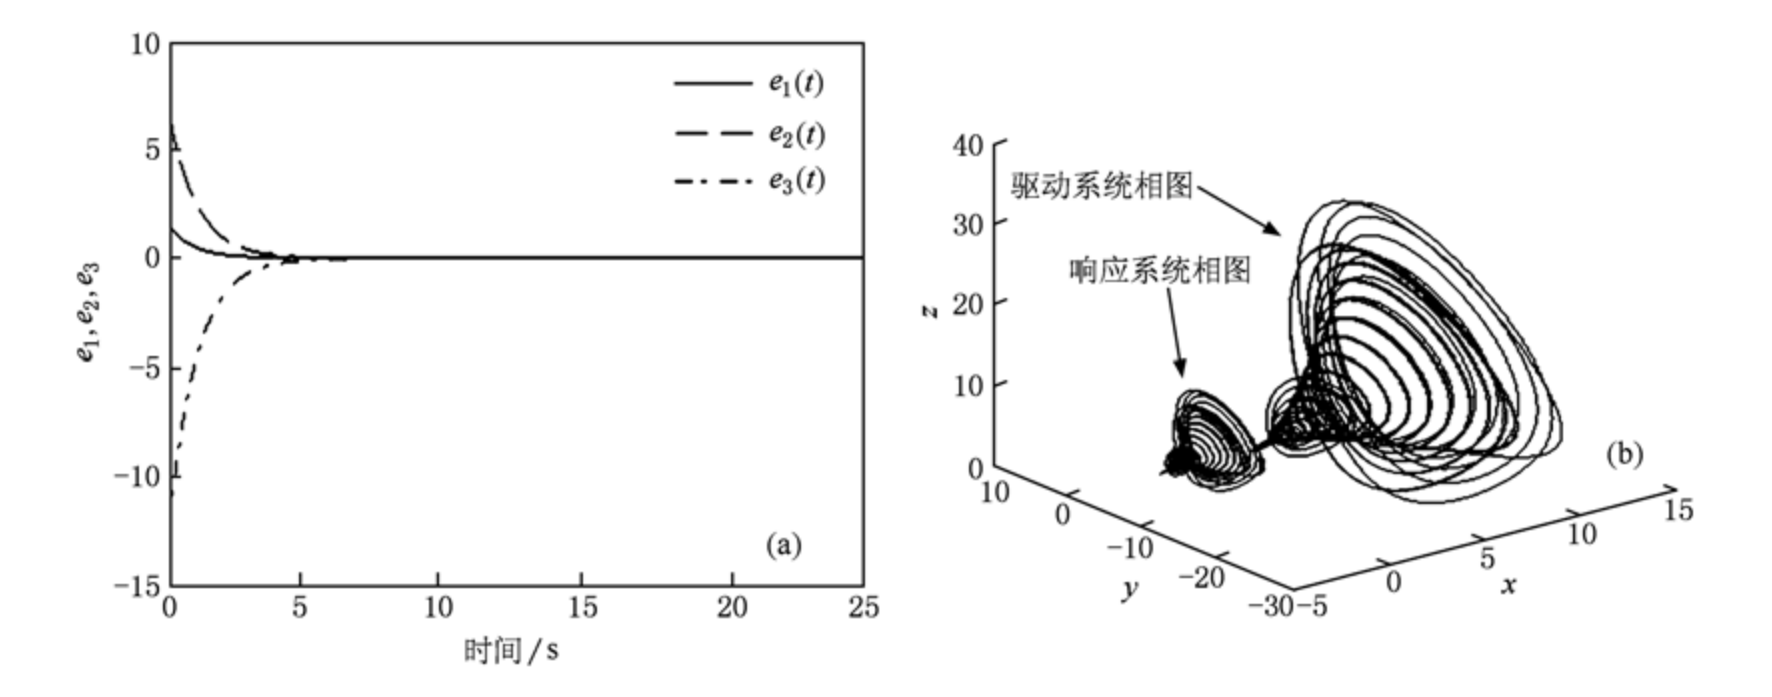
\includegraphics[width=0.9\textwidth,height=0.42\textheight,keepaspectratio]{aps2011-fig3.png}
\caption{(a) Synchronization error curves for $\alpha=3$; (b) three-dimensional GPS phase portraits for $\alpha=3$, showing in-phase compression.}
\label{fig:fig3}
\end{figure}

\section{Example 2: Heterostructure Synchronization (Energy System $\to$ NSG)}

The energy resource system drives a structurally different \textbf{Nuclear Spin Generator (NSG)} system:
\begin{equation}
\dot{x}_s = -a_3 x_s + y_s + u_1,
\qquad
\dot{y}_s = -x_s - a_3 y_s(1-b_4 z_s) + u_2,
\qquad
\dot{z}_s = c_4 a_3(1-z_s) - a_3 b_4 y_s^2 + u_3,
\label{eq:nsg}
\end{equation}
demonstrating that the modified active control works for \textbf{heterostructure} GPS --- the drive and response systems share neither structure nor parameter set.

\begin{figure}[htbp]
\centering
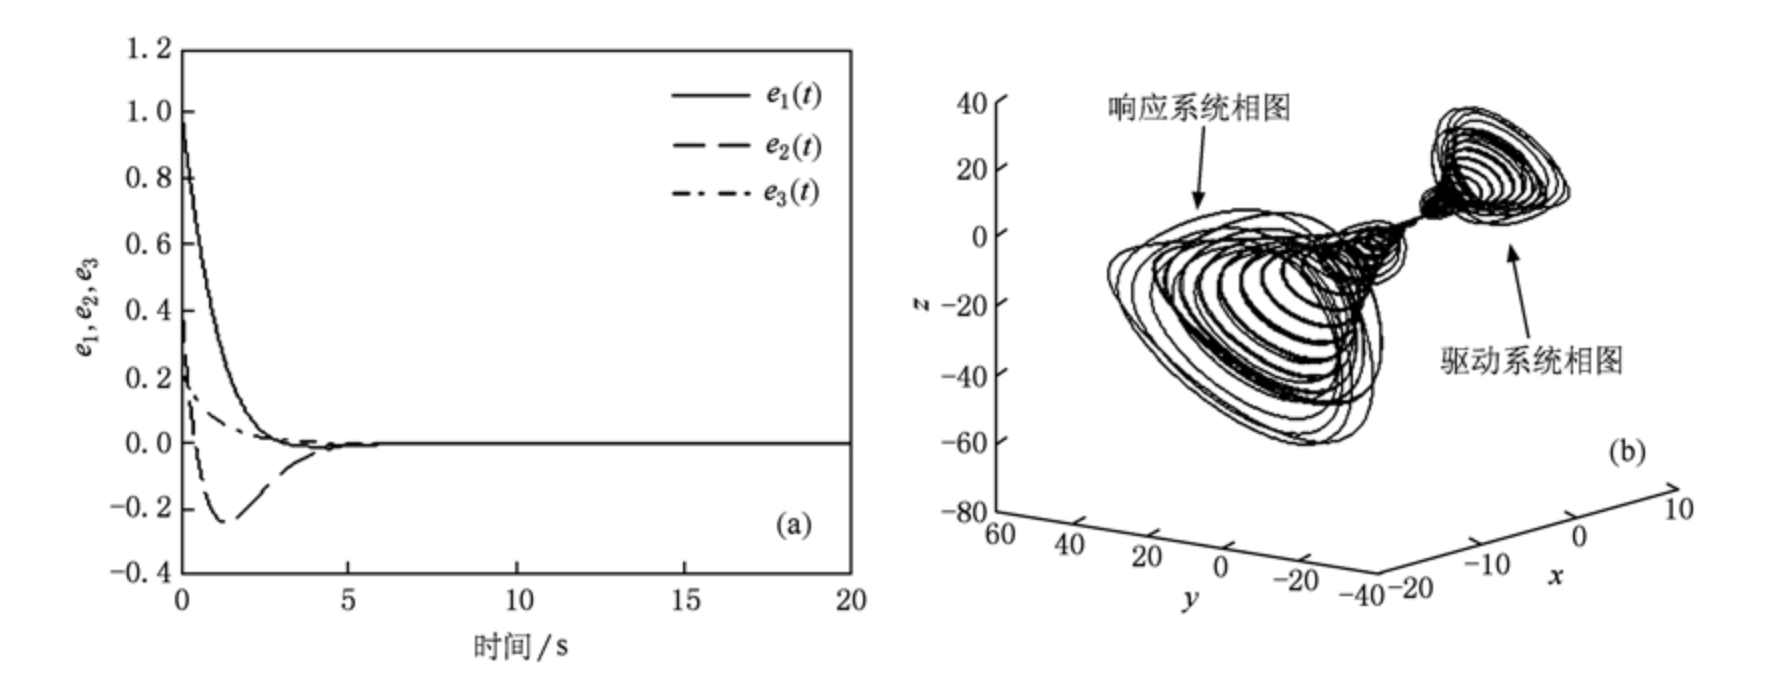
\includegraphics[width=0.9\textwidth,height=0.42\textheight,keepaspectratio]{aps2011-fig4.png}
\caption{(a) Heterostructure synchronization error for $\alpha=-0.5$ (anti-phase stretch); (b) three-dimensional GPS phase portraits for $\alpha=-0.5$.}
\label{fig:fig4}
\end{figure}

\begin{figure}[htbp]
\centering
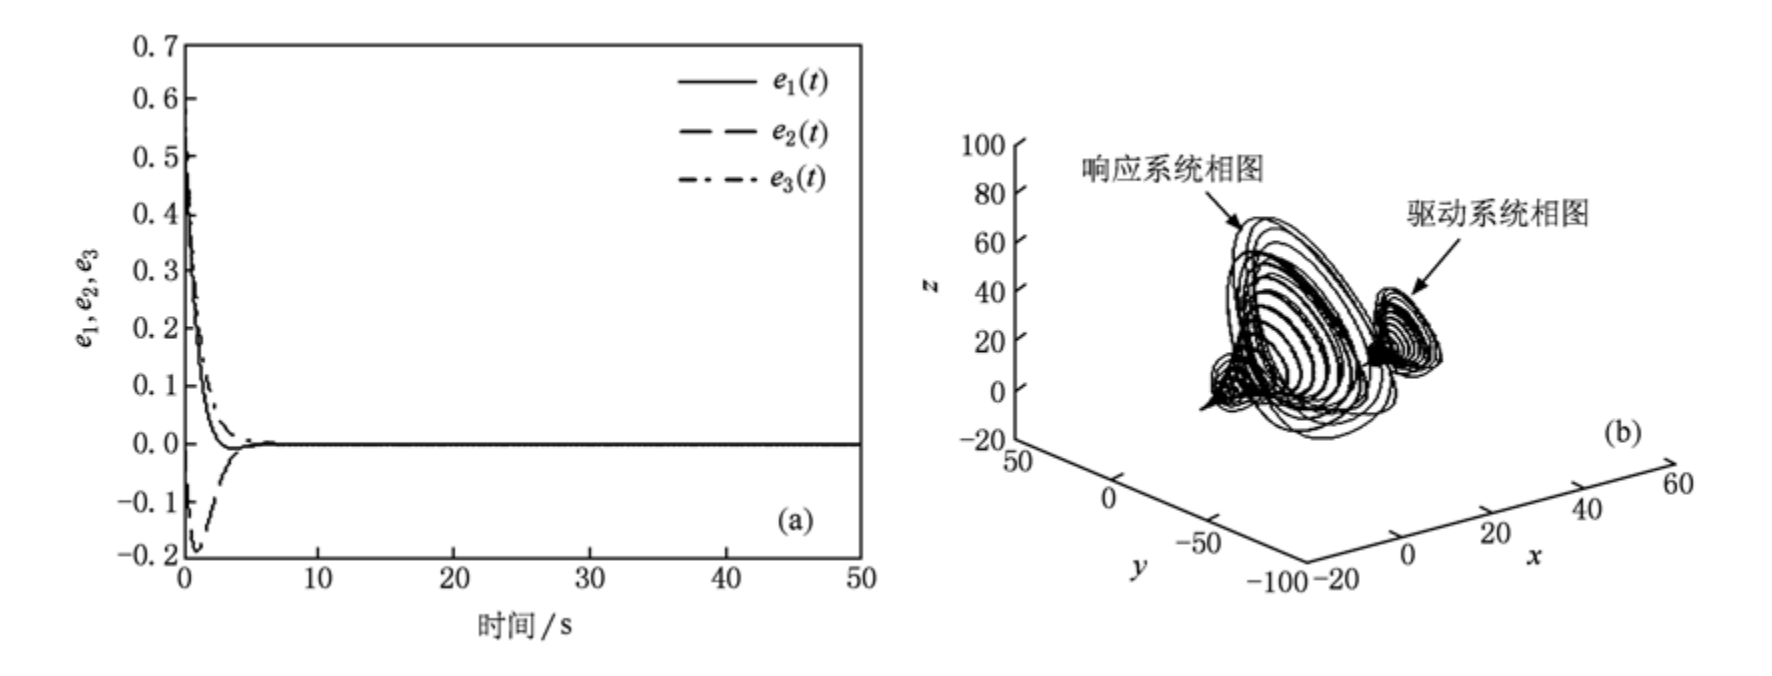
\includegraphics[width=0.9\textwidth,height=0.42\textheight,keepaspectratio]{aps2011-fig5.png}
\caption{(a) Heterostructure synchronization error for $\alpha=0.4$ (in-phase stretch); (b) three-dimensional GPS phase portraits for $\alpha=0.4$.}
\label{fig:fig5}
\end{figure}

The scaling law is complete: $-1<\alpha<0$ gives anti-phase stretching, $0<\alpha<1$ in-phase stretching, and $\alpha=\pm1$ recovers complete and anti-phase synchronization as special cases.

\section{Comparison with Tracking Control}

Figure~\ref{fig:fig6} shows the synchronization error produced by the classical tracking-control approach for the same drive--response pair ($\alpha=-0.5$). Compared with Figure~\ref{fig:fig4}(a), the modified active control converges \textbf{noticeably faster}, confirming its higher synchronization efficiency.

\begin{figure}[htbp]
\centering
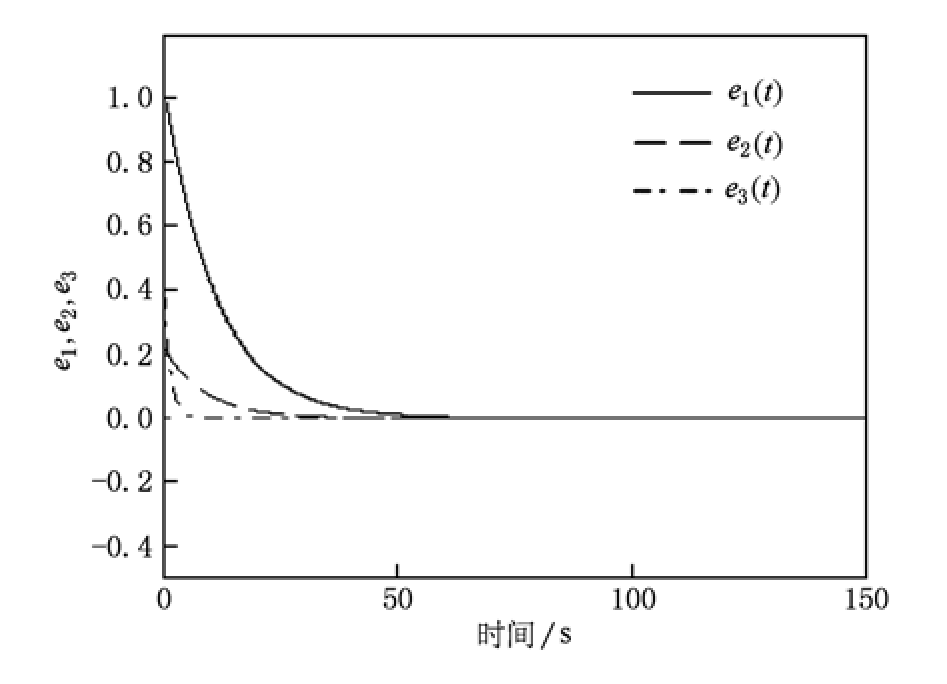
\includegraphics[width=0.8\textwidth,height=0.4\textheight,keepaspectratio]{aps2011-fig6.png}
\caption{Synchronization error curves under the tracking-control method. Faster convergence in the modified active control demonstrates its efficiency advantage.}
\label{fig:fig6}
\end{figure}

\section{Key Findings}

\begin{enumerate}[leftmargin=2em]
\item \textbf{Routh--Hurwitz independence (core contribution):} By constructing a special matrix $M$ so that the closed-loop matrix $N=E-M$ is skew-symmetric off-diagonal with non-positive diagonal, global GPS is guaranteed through the Lyapunov function Eq.~\eqref{eq:lyap} \emph{without} computing eigenvalues. This dramatically simplifies high-dimensional synchronization design.

\item \textbf{Universal applicability:} The method is validated for both self-structure GPS (energy system, $\alpha=-2,3$) and heterostructure GPS (energy system $\to$ NSG system, $\alpha=-0.5,0.4$), and works for low- and high-dimensional systems alike.

\item \textbf{Flexible scaling:} Tuning $\alpha$ realizes arbitrary in-phase/anti-phase compression or stretching of the drive signal --- a property valuable for secure communications.

\item \textbf{Higher efficiency than tracking control:} Error convergence under modified active control is faster than under tracking control, while retaining the robustness and simplicity of classical active control.

\item \textbf{Theoretical--numerical agreement:} All numerical simulations confirm the theoretical analysis, establishing the method's reliability.
\end{enumerate}

\section{Significance}

This paper represents the author's early work in nonlinear dynamics, centered on \textbf{chaos synchronization and control}. The two technical ingredients --- Lyapunov stability analysis and structured matrix construction --- later informed the author's development of analytical perturbation methods (the GHFP/MGHFP series). The paper also illustrates a general principle: for synchronization control, a well-chosen Lyapunov function can replace expensive algebraic criteria such as Routh--Hurwitz, making controller design simultaneously simpler and more transparent.

\vfill
\begin{center}
\small\rule{0.5\textwidth}{0.3pt}\\[4pt]
\small\color{primary} Author: Zhenbo Li (lizhenbo@usc.edu.cn)\\
\small ORCID: 0000-0003-2290-971X\\
\small University of South China, School of Mathematics and Physics\\
\small Hunan Key Laboratory of Mathematical Modeling and Scientific Computing
\end{center}

\end{document}
